\let\negmedspace\undefined
\let\negthickspace\undefined
\documentclass[journal]{IEEEtran}
\usepackage[a5paper, margin=10mm, onecolumn]{geometry}
%\usepackage{lmodern} % Ensure lmodern is loaded for pdflatex
\usepackage{tfrupee} % Include tfrupee package

\setlength{\headheight}{1cm} % Set the height of the header box
\setlength{\headsep}{0mm}     % Set the distance between the header box and the top of the text

\usepackage{gvv-book}
\usepackage{gvv}
\usepackage{cite}
\usepackage{amsmath,amssymb,amsfonts,amsthm}
\usepackage{algorithmic}
\usepackage{graphicx}
\usepackage{textcomp}
\usepackage{xcolor}
\usepackage{txfonts}
\usepackage{listings}
\usepackage{enumitem}
\usepackage{mathtools}
\usepackage{gensymb}
\usepackage{comment}
\usepackage[breaklinks=true]{hyperref}
\usepackage{tkz-euclide} 
\usepackage{listings}
% \usepackage{gvv}                                        
\def\inputGnumericTable{}                                 
\usepackage[latin1]{inputenc}                                
\usepackage{color}                                            
\usepackage{array}                                            
\usepackage{longtable}                                       
\usepackage{calc}                                             
\usepackage{multirow}                                         
\usepackage{hhline}                                           
\usepackage{ifthen}                                           
\usepackage{lscape}

\begin{document}

\bibliographystyle{IEEEtran}
\vspace{3cm}

\title{9-9.4-2}
\author{EE24BTECH11014 -DEEPAK}
% \maketitle
% \newpage
% \bigskip
{\let\newpage\relax\maketitle}

\renewcommand{\thefigure}{\theenumi}
\renewcommand{\thetable}{\theenumi}
\setlength{\intextsep}{10pt} % Space between text and floats


\numberwithin{equation}{enumi}
\numberwithin{figure}{enumi}
\renewcommand{\thetable}{\theenumi}
\textbf{Question}:\\
Find the area of the circle $ 4x^2 + 4y^2 = 9$ which is interior to the parabola $x^2 = 4y.$
\\
\solution
\begin{table}[h!]    
  \centering
  \begin{tabular}[12pt]{ |c| c|}
    \hline
    \textbf{Variable} & \textbf{Description}\\ 
    \hline
    $V_1,u_1,f_1$ & Parameters of Parabola \\
    \hline 
    $V_2,u_2,f_2$ & Parameters of circle \\
    \hline
     $P_1,P_2$ & Points of intersection \\
     \hline
     $A$ & Area between the conics \\
    \hline
\end{tabular}

  \caption{Variables Used}
\end{table}
The parameters of the conics are
\begin{align}
V_1=\myvec{0 & 0 \\ 0 & 1}\;,\;u_1=\myvec{0\\-2} \;,\;f_1=0\\
V_2=\myvec{1 & 0 \\ 0 & 1}\;,\;u_2=\myvec{0\\0}\;,\;f_2=-\frac{9}{4}
\end{align}
The intersection of two conics with parameters $V_i,u_i,f_i,\;i= 1,2$ is defined as
\begin{align}
x^T\brak{V_1+\mu V_2}x+2\brak{u_1+\mu u_2}^T x + \brak{f_1+\mu f_2}\;=\;0
\end{align}
Solving this the points of intersection are
\begin{align}
\myvec{\sqrt{2}\\\frac{1}{2}}\;,\myvec{-\sqrt{2}\\\frac{1}{2}}
\end{align}
Area between the curves is,
\begin{align}
2\int_{0}^{\frac{1}{2}} \brak{\sqrt{\frac{9}{4}-y^2}-\sqrt{4y}} \, dy 
\end{align}
By solving the integration, we get area is equal to 3.005 sq.units
\begin{figure}[h!]
   \centering
   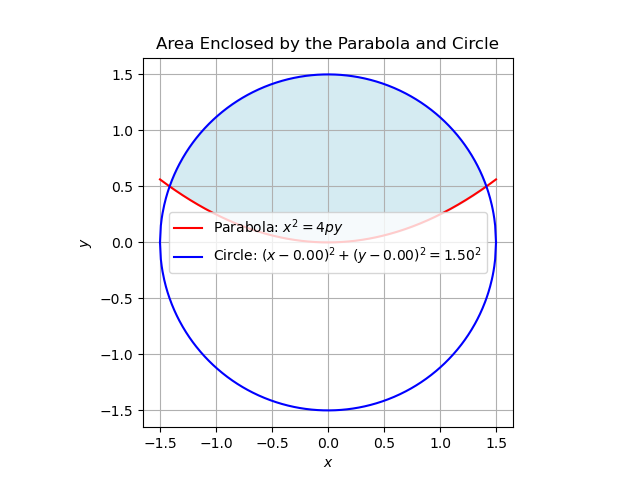
\includegraphics[width=\linewidth]{figs/fig2.png}
   \label{stemplot}
   \caption{}
\end{figure}


\end{document}




